Att exekvera ett program symboliskt innebär att representera värden utefter
programflödet som symboliska restriktioner (jfr eng.\ \emph{constraints}), vilka kan
lösas av automatiserade teoremlösare (\emph{SMT solver}). En symbolisk körning
representerar flera konkreta körningar eftersom de (symboliska) värden som
används representerar grupper av konkreta värden vilka har gemensamt hur de
påverkar programmets flöde~\cite{klee}.

Vägar i programmets kontrollflöde utforskas med symboliska uttryck som kallas
för path constraints (jfr sv.\ vägvillkor) för de begränsningar som finns på
programmets variabler --- vilka egenskaper de måste uppnå för att just denna väg
ska kunna följas~\cite{klee}. Huruvida villkorsblock av program är nårbara kan
evalueras eftersom de krav som måste uppfyllas för att följa vägen dit dokumenteras
under den symboliska körningen, och resulterar i fullständiga symboliska representationer
som en automatiserad teoremlösare (jmf.\ engelska SMT solver) kan appliceras på.

Eftersom de symboliska värdena har kapacitet att representera grupperingar av konkreta
värden istället för enskilda sådana, utförs en generaliserad testning av programmet,
som ger insikt i hur programmet beter sig givet en grupp av parametrar som alla
på grund av någon eller några gemensamma egenskaper, orsakar gemensamma beteenden
i programmet~\cite{Cadar}.

En symbolisk exekveringsmotor arbetar genom att först representera programmets
input som symboliska variablar, vilka vid starten inte har några begränsningar.
När programflödet når en branch som baseras på någon av de symboliska
variablerna, väljer motorn en branch och tillsätter dess path constraint på den
symboliska variabeln för alla vägar som fortsätter utefter branchen. Operationer
på värden under körningens väg översätts till symboliska operationer på
motsvarande symboliska variabler. När körning utefter branchen är
slutförd repeterar motorn samma metodik på samma branch för att utforska andra
alternativ. De tillståndsvillkor som en viss väg visas ha byggs därför
successivt upp genom att motorn utökar de symboliska variablerna till
villkorliga uttryck allt eftersom vägen följs~\cite{klee}.

Eftersom symbolisk exekvering kan leda till \emph{path explosion}, vilket
uppstår i program vars branches växer exponentiellt och resulterar i att en
symbolisk exekvering aldrig terminerar~\cite{path_explo}, är det inte effektivt
att alltid undersöka alla branchar i ett program. Exempel på metoder för att
undvika path explosion är \emph{state-merging} och \emph{heuristics}.

\begin{figure}
    \begin{lstlisting}[language=Python, frame=single]
x = input()
y = input()
z = 2 * y

if x == 100000:
  if x < z:
  # fabricated scenario of
  # memory vulnerability
    error_leading_to_mem_vuln()
  else:
    run_other_important_code()
else:
  run_important_code()

\end{lstlisting}
    \caption{Pseudokod för att visualisera symbolisk exekvering.}
    \label{fig:symbex_example_code}
\end{figure}

Exempletprogrammet i figur~\ref{fig:symbex_example_code} använder
symbolisk exekvering för att hitta vilken input som leder till de olika
vägarna. I många fall är det intressant att göra en uttömmande
sökning och hitta alla möjliga vägar i ett program, något som är möjligt i detta
program men inte alla program. Variablerna x och y sätts till symboliska värden
som sedan används för att beräkna path constraint och de symboliska uttryck som
variablerna utvecklas till för en vald branch. Därefter används dessa uttryck
och path constraint tillsammans för att bilda en ekvation som kan lösas med
hjälp av en SMT-solver och därmed få ut ett konkret värde.
Figur~\ref{fig:symbex_example_graph} visar hur det symboliska tillståndet
förändras för alla möjliga branches i programmet.

\begin{figure}
    \centering
    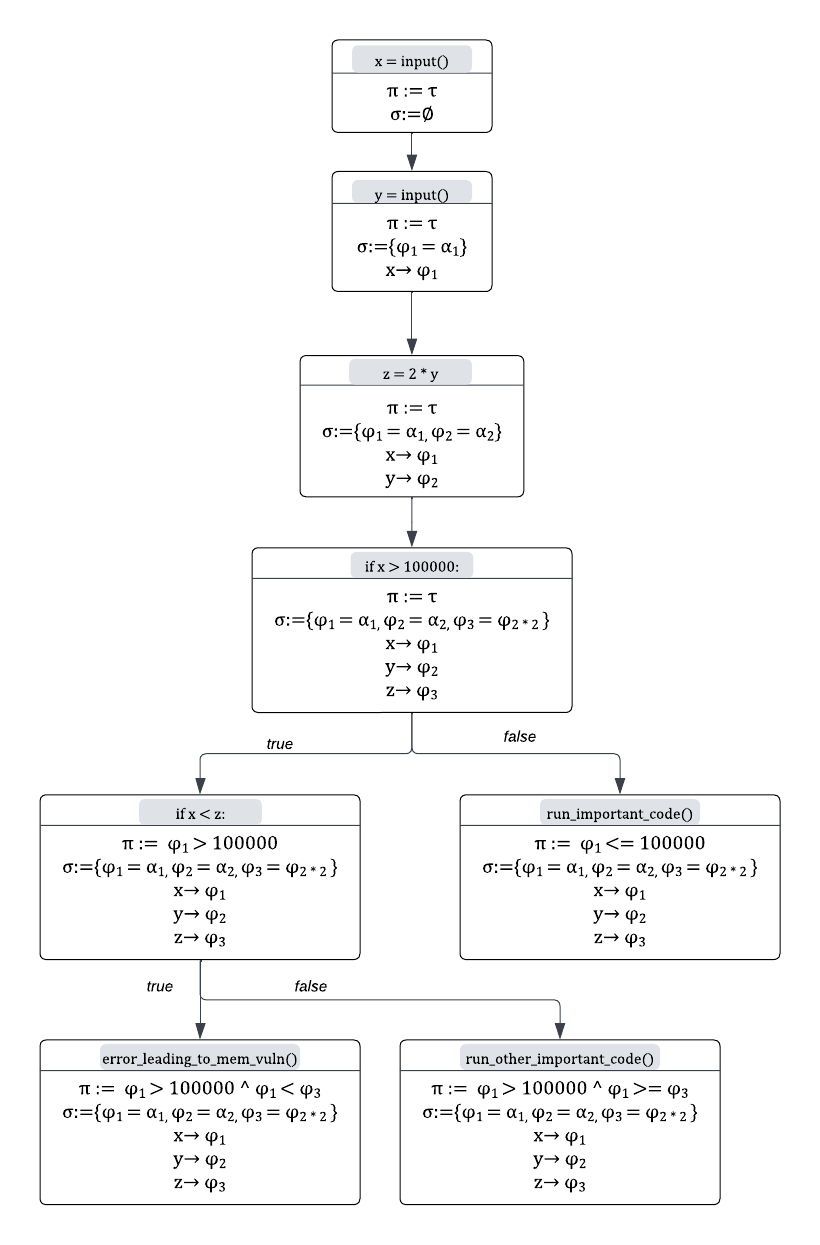
\includegraphics[scale=0.5]{figures/final_symbolic_example_graph.png}
    \caption{Path constraint och symboliskt tillstånd för alla stigar i
        pseudokoden angett i figur~\ref{fig:symbex_example_code}.}
    \label{fig:symbex_example_graph}
\end{figure}

I figur~\ref{fig:symbex_example_graph} används $\pi$ för att ange path constraint vilket
är initialt satt till $\top$ eftersom villkoret är sant från början och $\phi$
används för att visa mappningen för symboliska värden.

\todo[inline]{Explain a bit the graphs in figure \ref{fig:symbex_example_graph} and how
    elements of each node are constructed, no need to do it for all nodes,  but for
    1, 2, 4 and explain the path split // Iulia}
